\documentclass[12pt,a4paper]{article}
\usepackage{amsmath,amsthm,amsfonts,tikz}
\usepackage{algorithm,algpseudocode}
\usepackage[margin=2cm]{geometry}
\usepackage[euler-digits]{eulervm}
\usepackage{hyperref}
\usepackage[capitalize]{cleveref}
%%%%%%%%%%%%%%%%%%%%%%%%%%%%%%%%%%%%%%%%%%%%%%%%%%%%%%%%%%%%%%%%%%%%%
\newtheorem{theorem}{Theorem}
\newtheorem{corollary}[theorem]{Corollary}
\newtheorem{lemma}[theorem]{Lemma}
\newcommand{\iprod}[1]{\langle#1\rangle}
\newcommand{\vecp}[1]{\boldsymbol{p}}
\newcommand{\hatvecp}{\hat{\boldsymbol{p}}}
\newcommand{\Poly}{\mathbb{P}}
\newcommand{\bs}[1]{\boldsymbol{#1}}
\newcommand{\vecspan}{\operatorname{span}}
\newcommand{\sign}{\mathrm{sign}}
%%%%%%%%%%%%%%%%%%%%%%%%%%%%%%%%%%%%%%%%%%%%%%%%%%%%%%%%%%%%%%%%%%%%%
\title{Notes on Gauss Quadrature for General Weight Functions}
\author{Bill McLean}
\date{\today}
%%%%%%%%%%%%%%%%%%%%%%%%%%%%%%%%%%%%%%%%%%%%%%%%%%%%%%%%%%%%%%%%%%%%%
\begin{document}
\maketitle
\tableofcontents
%%%%%%%%%%%%%%%%%%%%%%%%%%%%%%%%%%%%%%%%%%%%%%%%%%%%%%%%%%%%%%%%%%%%%
\section{Three-term recurrence relation}
Let $\Poly_k$ denote the $(k+1)$-dimensional vector space of real 
polynomials with degree at most~$k$, and denote the 
infinite-dimensional space of all polynomials by~$\Poly$.  Let $\mu$ 
be a positive measure on the real line with the property that if
$\int f(x)^2\,d\mu(x)=0$~and $f\in\Poly$ then $f=0$.
We can then define an inner product and norm on~$\Poly$  by
\[
\iprod{f,g}=\int f(x)g(x)\,d\mu(x)\quad\text{and}\quad
\|f\|=\sqrt{\iprod{f,f}}.
\]
Using the Gram--Schmidt procedure to orthogonalise the linearly 
independent monomials $1$, $x$, $x^2$, $x^3$, \dots, yields a
polynomial of degree~$j$,  
\[
p_j(x)=x^j-\sum_{k=0}^{j-1}\frac{\iprod{x^j,p_k}}{\|p_k\|^2}\,p_k(x)
	\quad\text{for $j=0$, $1$, $2$, \dots.}
\]
Therefore, $p_j$ is the unique monic polynomial in~$\Poly_j$ such 
that $p_j\perp\Poly_{j-1}$; in particular,
\begin{equation}\label{eq: orthog}
\iprod{p_j,p_k}=0\quad\text{if $j\ne k$.}
\end{equation}

\begin{theorem}\label{thm: 3 term}
The orthogonal polynomials defined above satisfy the three-term 
recurrence relation
\begin{equation}\label{eq: 3 term pj}
p_j(x)=(x-a_j)p_{j-1}(x)-b_{j-1}^2p_{j-2}(x)
	\quad\text{for $j=1$, $2$, $3$, \dots,}
\end{equation}
with $p_0(x)=1$ and $p_{-1}(x)=0$. The coefficients satisfy
\[
a_j=\frac{\iprod{xp_{j-1},p_{j-1}}}{\|p_{j-1}\|^2}
\quad\text{and}\quad
b_j=\frac{\|p_j\|}{\|p_{j-1}\|},
\]
except that, by convention, we put $b_0=\|p_0\|=\sqrt{\int\,d\mu}$.
\end{theorem}
\begin{proof}
Since $p_j(x)-xp_{j-1}(x)$ has degree at most~$j-1$, there are 
constants~$c_{jk}$ such that
\[
p_j(x)-xp_{j-1}(x)=\sum_{k=0}^{j-1}c_{jk}p_k(x).
\]
Taking the inner product of both sides with~$p_{j-1}$ and using
the orthogonality property~\eqref{eq: orthog}, we obtain
\[
-\iprod{xp_{j-1},p_{j-1}}=c_{j,j-1}\|p_{j-1}\|^2,
\]
showing that $c_{j,j-1}=-a_j$.  Also, taking the inner product of both
sides with~$p_k$ for $k\le j-3$ gives
\[
c_{jk}\|p_k\|^2=\iprod{p_j-xp_{j-1},p_k}=-\iprod{p_{j-1},xp_k}=0,
\]
so 
\[
p_j(x)-xp_{j-1}(x)=\sum_{k=j-2}^{j-1}c_{jk}p_k(x)
	=-a_jp_{j-1}(x)+c_{j,j-2}p_{j-2}(x).
\]
Hence,
\[
p_j(x)=(x-a_j)p_{j-1}(x)+c_{j,j-2}p_{j-2}(x)
\]
and
\[
0=\iprod{p_j,p_{j-2}}=\iprod{xp_{j-1},p_{j-2}}+c_{j,j-2}\|p_{j-2}\|^2.
\]
Finally, since $xp_{j-2}-p_{j-1}\in\Poly_{j-2}$,
\[
\iprod{xp_{j-1},p_{j-2}}=\iprod{p_{j-1},xp_{j-2}}
	=\iprod{p_{j-1},p_{j-1}}+\iprod{p_{j-1},xp_{j-2}-p_{j-1}}
	=\|p_{j-1}\|^2+0,
\]
and therefore $c_{j,j-2}=-\|p_{j-1}\|^2/\|p_{j-2}\|^2=-b_{j-1}^2$.
\end{proof}

\begin{corollary}
$\|p_j\|=b_0b_1\cdots b_j$ for $j=1$, $2$, $3$, \dots.
\end{corollary}

Recall that the Lagrange interpolation polynomial
\[
\ell_j(x)=\prod_{\substack{k=1\\ k\ne j}}^n\frac{x-x_k}{x_j-x_k}.
\]
has the property that $\ell_j(x_k)=\delta_{jk}$. The zeros of~$p_n$ 
have the following important properties.  

\begin{theorem}
Suppose that $d\mu(x)=w(x)\,dx$ with $w(x)>0$ for $a<x<b$.
(We allow $a=-\infty$ or $b=\infty$.) The orthogonal polynomial has 
only real and simple zeros~$x_j$ in the open interval~$(a,b)$, that 
is,
\[
a<x_1<x_2<\cdots<x_n<b.
\]
\end{theorem}
\begin{proof}
Suppose for a contradiction that $p_n$ has a zero $\alpha+i\beta$ 
with~$\beta\ne0$.  Since $p_n$ has real coefficients, 
the complex conjugate~$\alpha-i\beta$ is also a zero and thus
\[
p_n(x)=\bigl[x-(\alpha+i\beta)\bigr]\bigl[x-(\alpha-i\beta)\bigr]q(x)
	=[(x-\alpha)^2+\beta^2]q(x)
\]
with $n\ge2$~and $q\in\Poly_{n-2}$. Since $p_n\perp\Poly_{n-2}$,
\[
0=\iprod{p_n,q}=\iprod{[(x-\alpha)^2+\beta^2]q,q}\\
	=\|(x-\alpha)q\|^2+\beta^2\|q\|^2,
\]
implying that $q=0$ and thus $p_n=0$, a contradiction.

Likewise, suppose for a contradiction that $p_n$ has a multiple real 
root~$\alpha$ and write $p_n(x)=(x-\alpha)^2q(x)$ with 
$q\in\Poly_{n-2}$.  Then
\[
0=\iprod{p_n,q}=\iprod{(x-\alpha)^2q,q}=\|(x-\alpha)q\|^2,
\]
again implying that $q=0$ and thus $p_n=0$.  We conclude that $p_n$ 
has only distinct real zeros~$x_j$.

Thus, for $1\le j\le n$,
\[
p_n(x)=\prod_{k=1}^n(x-x_k)=c_j(x-x_j)\ell_j(x)
\quad\text{where}\quad
c_j=\prod_{\substack{k=1\\ k\ne j}}^n(x_j-x_k)\ne0.
\]
Since $\ell_j\in\Poly_{n-1}$ and $p_n\perp\Poly_{n-1}$,
\[
0=\iprod{p_n,\ell_j}=\iprod{c_j(x-x_j)\ell_j,\ell_j}
	=c_j\bigl[(x\ell_j,\ell_j)-x_j\|\ell_j\|^2\bigr],
\]
implying that
\[
x_j=\frac{\iprod{x\ell_j,\ell_j}}{\|\ell_j\|^2}.
\]
By integrating the strict inequalities
\[
a\ell_j(x)^2w(x)<x\ell_j(x)^2w(x)<b\ell_j(x)^2w(x)
	\quad\text{for $a<x<b$,}
\]
we see that $a\|\ell_j\|^2<\iprod{x\ell_j,\ell_j}<b\|\ell_j\|^2$
and therefore $a<x_j<b$, as claimed.
\end{proof}

We denote the ortho\emph{normal} polynomials by
\[
\hat p_j(x)=\frac{p_j(x)}{\|p_j\|},
\]
and find that
\begin{equation}\label{eq: p hat recurrence}
b_j\hat p_j(x)=(x-a_j)\hat p_{j-1}(x)-b_{j-1}\hat p_{j-2}(x),
\end{equation}
or equivalently,
\begin{equation}\label{eq: 3 term orthog}
b_{j-1}\hat p_{j-2}(x)+a_j\hat p_{j-1}(x)+b_j\hat p_j(x)=xp_{j-1}(x).
\end{equation}

\begin{theorem}[Christoffel--Darboux identity]
\label{thm: Christoffel-Darboux}
The monic orthogonal polynomials satisfy
\[
\frac{1}{b_{n+1}}\sum_{k=0}^n\hat p_k(x)\hat p_k(y)
	=\frac{\hat p_{n+1}(x)\hat p_n(y)-\hat p_n(x)\hat p_{n+1}(y)}{x-y}
	\quad\text{for $x\ne y$.}
\]
\end{theorem}
\begin{proof}
Using \eqref{eq: 3 term orthog}, we see that
\begin{align*}
(x-y)\hat p_{k-1}(x)&\hat p_{k-1}(y)
	=[x\hat p_{k-1}(x)]\hat p_{k-1}(y)
		-\hat p_{k-1}(x)[y\hat p_{k-1}(y)]\\
	&=\bigl[
	b_{k-1}\hat p_{k-2}(x)+a_k\hat p_{k-1}(x)+b_k\hat p_k(x)
	\bigr]\hat p_{k-1}(y)\\
	&\qquad{}-\hat p_{k-1}(x)\bigl[
	b_{k-1}\hat p_{k-2}(y)+a_k\hat p_{k-1}(y)+b_k\hat p_k(y)\bigr]\\
	&=\bigl[b_{k-1}\hat p_{k-2}(x)\hat p_{k-1}(y)
		-b_k\hat p_{k-1}(x)\hat p_k(y)\bigr]\\
	&\qquad{}+\bigl[b_k\hat p_k(x)\hat p_{k-1}(y)
		-b_{k-1}\hat p_{k-1}(x)\hat p_{k-2}(y)\bigr]\\
\end{align*}
and so
\begin{align*}
(x-y)\smash[b]{\sum_{k=1}^{n+1}}\hat p_{k-1}(x)\hat p_{k-1}(y)
	&=b_0\hat p_{-1}(x)\hat p_0(y)-b_{n+1}\hat p_n(x)\hat p_{n+1}(y)\\
	&\qquad{}+b_{n+1}\hat p_{n+1}(x)\hat p_n(y)
		-b_0\hat p_0(x)\hat p_{-1}(y),
\end{align*}
which implies the desired formula since $p_{-1}(x)=0$.
\end{proof}


\subsection{Legendre polynomials}
The Legendre polynomials have the orthogonality property
\begin{equation}\label{eq: legendre orthog}
\int_{-1}^1 P_j(x)P_k(x)\,dx=\frac{2\delta_{jk}}{2j+1}
\end{equation}
and the 3-term recurrence relation is
\begin{equation}\label{eq: legendre 3 term}
jP_j(x)=(2j-1)xP_{j-1}(x)-(j-1)P_{j-2}(x).
\end{equation}
The normalised Legendre polynomials are
\[
\hat P_j(x)=\frac{P_j(x)}{\|P_j\|}=\biggl(\frac{2j+1}{2}\biggr)^{1/2}
	P_j(x),
\]
and thus
\[
j\biggl(\frac{2}{2j+1}\biggr)^{1/2}\hat P_j(x)
	=(2j-1)\biggl(\frac{2}{2j-1}\biggr)^{1/2}x\hat P_{j-1}(x)\\
	-(j-1)\biggl(\frac{2}{2j-3}\biggr)^{1/2}\hat P_{j-2}(x),
\]
or equivalently,
\[
\frac{j\hat P_j(x)}{\sqrt{2j+1}}=\sqrt{2j-1}\,x\hat P_{j-1}(x)
	-\frac{k-j}{\sqrt{2j-3}}\,\hat P_{j-2}(x).
\]
Thus, 
\[
b_j\hat P_j(x)=(x-a_j)\hat P_{j-1}(x)-b_{j-1}\hat P_{j-2}(x)
\]
where
\[
a_j=0\quad\text{and}\quad b_j=\frac{j}{\sqrt{(2j-1)(2j+1)}},
\]
except that $b_0=\sqrt{\int_{-1}^1\,dx}=\sqrt{2}$.

\section{Gauss quadrature}
We now consider a quadrature rule
\begin{equation}\label{eq: Qf}
Qf=\sum_{j=1}^n w_jf(x_j)
\end{equation}
and its associated error functional
\[
Ef=\int f(x)\,d\mu(x)-\sum_{j=1}^n w_jf(x_j).
\]

\begin{theorem}\label{thm: Gauss rule}
For each $n\ge1$ there exists a unique quadrature rule~\eqref{eq: Qf}
such that
\begin{equation}\label{eq: dop 2n-1}
Ef=0\quad\text{for all $f\in\Poly_{2n-1}$.}
\end{equation}
This rule has has as its integration points $x_1$, $x_2$, \dots, 
$x_n$ the zeros of~$p_n$, that is,
\[
p_n(x_j)=0\quad\text{for $1\le j\le n$,}
\]
and as its weights the numbers
\begin{equation}\label{eq: Gauss weights}
w_j=\iprod{\ell_j,1}=\|\ell_j\|^2>0
	\quad\text{for $1\le j\le n$,}
\end{equation}
where $\ell_j$ is the $j$th Lagrange interpolation polynomial:
\[
\ell_j(x)=\prod_{\substack{k=1\\ k\ne j}}\frac{x-x_k}{x_j-x_k}.
\]
\end{theorem}
\begin{proof}
Let $x_1$, $x_2$, \dots, $x_n$ be the zeros of~$p_n$, and define
$w_j=\iprod{\ell_j,1}$.  Given $f\in\Poly_{2n-1}$, let $q$~and $r$ 
denote the quotient and remainder when $f$ is divided by~$p_n$, that 
is,
\[
f(x)=p_n(x)q(x)+r(x)\quad\text{with $r\in\Poly_{n-1}$.}
\]
Since $p_n(x_j)=0$ it follows that $f(x_j)=r(x_j)$ and so
\[
r(x)=\sum_{j=1}^n f(x_j)\ell(x),
\]
and since $q\in\Poly_{n-1}$ and $p_n$ is orthogonal to~$\Poly_{n-1}$,
\begin{multline*}
\int f(x)\,d\mu(x)=\int q(x)p_n(x)\,d\mu(x)+\int r(x)\,d\mu(x)\\
	=\iprod{q,p_n}+\sum_{j=1}^n f(x_j)\int\ell_j(x)\,d\mu(x)
	=0+\sum_{j=1}^n f(x_j)\iprod{\ell_j,1}=Qf,
\end{multline*}
showing that $Ef=0$.  

To prove uniqueness, let $Q$ be any quadrature rule~\eqref{eq: Qf} 
satisfying \eqref{eq: dop 2n-1}.  Consider the 
polynomial~$f\in\Poly_n$ defined by
\[
f(x)=(x-x_1)(x-x_2)\cdots(x-x_n).
\]
If $0\le k\le n-1$ then $x^kf(x)\in\Poly_{2n-1}$ so
\[
\iprod{x^k,f}=\int x^kf(x)\,d\mu(x)=\sum_{j=1}^n w_jx_j^kf(x_j)=0.
\]
Hence, $f\perp\Poly_{n-1}$, and since $f$ is monic it follows that 
$f=p_n$ by the uniqueness of the orthogonal polynomials.  Therefore,
the $x_j$ are the zeros of~$p_n$, and moreover
\[
w_j=\sum_{k=1}^nw_k\ell_j(x_k)=\int\ell_k(x)\,d\mu(x)=\iprod{\ell_j,1}
\]
since $\ell_j\in\Poly_{n-1}$.  In fact, $\ell_j^2\in\Poly_{2n-2}$ so
\[
w_j=\sum_{k=1}^nw_k\ell_j(x_k)^2=\int\ell_j(x)^2\,d\mu(x)
	=\|\ell_j\|^2>0,
\]
and the weights satisfy~\eqref{eq: Gauss weights}.
\end{proof}

The quadrature method in the above theorem is called the $n$-point Gauss 
rule generated by the positive measure~$\mu$.

Defining
\[
T_n=\begin{bmatrix}
a_1&b_1   &       &       &\\
b_1&a_2   &b_2    &       &\\
   &\ddots&\ddots &\ddots &\\
   &      &b_{n-2}&a_{n-1}&b_{n-1}\\
   &      &       &b_{n-1}&a_n
\end{bmatrix}
\quad\text{and}\quad
\hatvecp_n(x)=\begin{bmatrix}
	\hat p_0(x)\\ \hat p_1(x)\\ \vdots\\ \hat p_{n-1}(x)
\end{bmatrix},
\]
the equations~\eqref{eq: 3 term orthog} for $0\le j\le n-1$ are 
equivalent to
\begin{equation}\label{eq: matrix 3 term orthog}
T_n\hatvecp_n(x)+b_n\hat p_n(x)\boldsymbol{e}_n=x\hatvecp_n(x).
\end{equation}
The points~$x_j$ and weights~$w_j$ may be computed by solving an 
eigenproblem for the \emph{Jacobi matrix}~$T_n$.

\begin{theorem}\label{thm: Jacobi eigenproblem}
The eigenvalues of~$T_n$ are the points $x_1$, $x_2$, \dots, $x_n$
of the associated Gauss quadrature rule.  Moreover, for~$1\le j\le n$,
if
\[
\boldsymbol{v}_j=\begin{bmatrix}v_{1j}\\ v_{2j}\\ \vdots\\ v_{nj}
\end{bmatrix}
\]
denotes the eigenvector of~$T_n$ satisfying
\[
T_n\boldsymbol{v}_j=x_j\boldsymbol{v}_j
\quad\text{and}\quad
v_{1j}=\frac{1}{b_0},
\]
then the weight~$w_j$ corresponding to the $j$th Gauss point~$x_j$ 
is given by
\[
\frac{1}{w_j}=\sum_{k=1}^n(v_{kj})^2.
\]
\end{theorem}
\begin{proof}
We see at once from~\eqref{eq: matrix 3 term orthog} that 
$T_n\hatvecp_n(x)=x\hatvecp_n(x)$ iff $p_n(x_j)=0$, so the
eigenvalues~$x_j$ of~$T_n$ coincide with zeros of~$p_n$ which,
by Theorem~\ref{thm: Gauss rule}, coincide with the Gauss points.  
Moreover, $\boldsymbol{v}_j=\hatvecp_n(x_j)$ is the eigenvector 
of~$T_n$ that corresponds to the eigenvalue~$x_j$ and is scaled in 
such a way that $v_{1k}=\hat p_0(x_j)=1/\|p_0\|=1/b_0$.

Since $p_n$ is monic with zeros $x_1$, $x_2$, \dots, $x_n$,
\[
p_n(x)=\prod_{j=1}^n(x-x_j)
\qquad\text{and thus}\qquad
p_n'(x)=\sum_{j=1}^n\prod_{\substack{k=1\\ k\ne j}}^n(x-x_k).
\]
In particular
\[
p_n'(x_j)=\prod_{\substack{k=1\\ k\ne j}}^n(x_j-x_k),
\]
showing that
\[
p_n(x)=p_n'(x_j)(x-x_j)\ell_j(x)\quad\text{where}\quad
\ell_j(x)=\prod_{\substack{k=1\\ k\ne j}}^n\frac{x-x_k}{x_j-x_k}.
\]
Hence, $\hat p_n(x)=\hat p_n'(x_j)(x-x_j)\ell_j(x)$ and so
\begin{equation}\label{eq: w_j}
w_j=\iprod{\ell_j,1}=\frac{1}{\hat p_n'(x_j)}
	\int\frac{\hat p_n(x)}{x-x_j}\,w(x)\,dx.
\end{equation}
Putting $y=x_j$ in the Christoffel--Darboux identity of 
Theorem~\ref{thm: Christoffel-Darboux} gives
\[
\frac{1}{b_{n+1}}\sum_{k=0}^n\hat p_k(x)\hat p_k(x_j)
	=-\frac{\hat p_n(x)}{x-x_j}\,\hat p_{n+1}(x_j)
\]
and after taking the inner product of both sides with~$p_0(x)=1$
we obtain
\[
\frac{1}{b_{n+1}}\sum_{k=0}^n\iprod{\hat p_k,p_0}\hat p_k(x_j)
	=-\hat p_{n+1}(x_j)\int_a^b\frac{\hat p_n(x)}{x-x_j}\,w(x)\,dx.
\]
Here, $\iprod{\hat p_k,p_0}=0$ for~$k\ge1$ and 
$\iprod{\hat p_0,p_0}\hat p_0(x_j)=\iprod{p_0/\|p_0\|,p_0}/\|p_0\|=1$, so
\[
\frac{1}{b_{n+1}}=-\hat p_{n+1}(x_j)\int\frac{\hat p_n(x)}{x-x_j}\,w(x)\,dx.
\]
Thus, by~\eqref{eq: w_j},
\[
\frac{1}{b_{n+1}}=-\hat p_{n+1}(x_j)\hat p_n'(x_j)w_j.
\]
The Christoffel--Darboux identity also gives
\begin{align*}
\frac{1}{b_{n+1}}\sum_{k=0}^n\hat p_k(x_j)^2
&=\lim_{y\to x_j}\frac{1}{b_{n+1}}\sum_{k=0}^n
	\hat p_k(x_j)\hat p_k(y)
=\lim_{y\to x_j}\frac{\hat p_{n+1}(x_j)\hat p_n(y)}{x_j-y}\\
&=-\hat p_{n+1}(x_j)\lim_{y\to x_j}
	\frac{\hat p_n(y)-\hat p_n(x_j)}{y-x_j}
	=-\hat p_{n+1}(x_j)\hat p_n'(x_j) 
\end{align*}
and therefore
\[
\frac{1}{w_j}=-b_{n+1}\hat p_{n+1}(x_j)\hat p_n'(x_j)
	=\sum_{k=0}^n\hat p_k(x_j)^2=\sum_{k=1}^n(v_{kj})^2,
\]
as claimed.
\end{proof}
\begin{corollary}
Let $\hat{\boldsymbol{v}}_j=\boldsymbol{v}_j/\|\boldsymbol{v}_j\|$ denote the 
$j$th normalised eigenvector.  Then, the Gauss quadrature weights are
\[
w_j=(b_0\hat v_{1j})^2\quad\text{for $1\le j\le n$.}
\]
\end{corollary}
\begin{proof}
We have $\|\boldsymbol{v}_j\|^2=\sum_{k=1}^n(v_{kj})^2=w_j^{-1}$ so
$(\hat v_{1j})^2=(v_{1j})^2/\|\boldsymbol{v}_j\|^2=w_j/b_0^2$.
\end{proof}



\section{The modified Chebyshev algorithm}

Let $q_0$, $q_1$, $q_2$, \dots be a sequence of monic orthogonal 
polynomials generated by a positive measure $\nu$ on the real line.  
Thus, $q_k\in\Poly_k$ is a monic polynomial satisfying 
\[
\int q_k(x)f(x)\,d\nu(x)=0\quad\text{for all $f\in\Poly_{k-1}$.}
\]
In the usual way, we write the three-term recurrence relation as
\begin{equation}\label{eq: 3 term q}
q_k(x)=(x-\alpha_k)q_{k-1}(x)-\beta_{k-1}^2 q_{k-2}(x)
	\quad\text{for $k=1$, $2$, $3$, \dots,}
\end{equation}
with
\[
q_0(x)=1\quad\text{and}\quad q_{-1}(x)=0,
\]
adopting the usual convention that $\beta_0=\|q_0\|_\nu=\sqrt{\int d\nu}$.  
Also, by~\eqref{eq: p hat recurrence}, the normalised orthogonal polynomials
$\hat q_k(x)=q_k(x)/\|q_k\|_\nu$ satisfy
\begin{equation}\label{eq: q hat recurrence}
\beta_k\hat q_k(x)=(x-\alpha_k)\hat q_{k-1}(x)-\beta_{k-1}\hat q_{k-1}(x)
\quad\text{for $k=1$, $2$, $3$, \dots.}
\end{equation}

Suppose that $p_0$, $p_1$, $p_2$, \dots is another sequence of monic 
orthogonal polynomials generated by a positive measure $\mu$ and 
having known coefficients $a_j$~and $b_j$ in the associated 
three-term recurrence relation~\eqref{eq: 3 term pj}; thus
\[
\int p_j(x)f(x)\,d\mu(x)=0\quad\text{for all $f\in\Poly_{j-1}$.}
\]
Following Gautschi~\cite{Gautschi1982}, we consider the case when 
$\alpha_k$~and $\beta_k$ are not known explicitly, but we are able to 
find the modified moments
\[
\nu_j=\int\hat p_j(x)\,d\nu(x)\quad\text{for $0\le l\le 2n-1$,}
\]
where, as usual, $\hat p_0$, $\hat p_1$, $\hat p_2$, \dots are the 
orthonormalised polynomials satisfying
\[
\int\hat p_j(x)\hat p_k(x)\,d\mu(x)=\delta_{jk}.
\]
The next theorem summarises the modified Chebyshev algorithm for 
computing $\alpha_k$~and $\beta_k$ for $1\le k\le n$.

\begin{figure}
\caption{The dots correspond to the $\sigma_{lk}$ computed in the 
case~$n=5$.  The parallelogram indicates the $\sigma_{lk}$ used in 
the expressions for $\alpha_5$~and $\beta_5$.}
\begin{center}
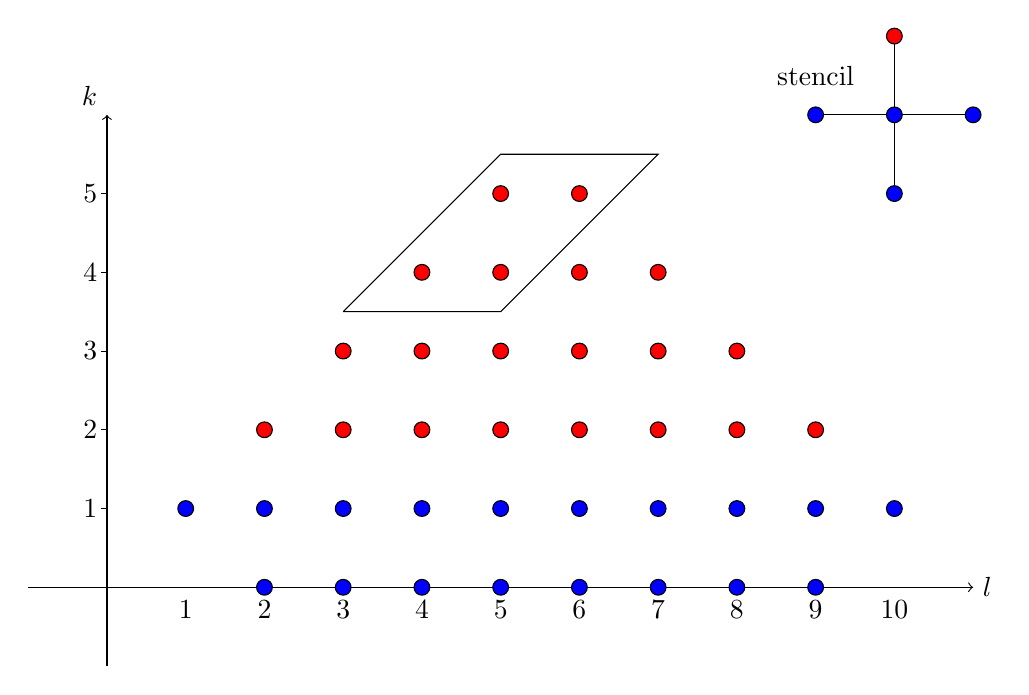
\begin{tikzpicture}[scale=1.0]
\draw[->] (0, -1) -- (0, 6);
\node[above left] at (0, 6) {$k$};
\draw[->] (-1, 0) -- (11, 0);
\node[right] at (11, 0) {$l$};
\foreach \x in {2, 3, ..., 9}
    \draw[fill=blue] (\x, 0) circle(0.10cm);
\foreach \x in {1, 2, ..., 10}
    \draw[fill=blue] (\x, 1) circle(0.10cm);
\foreach \x in {2, 3, ..., 9}
    \draw[fill=red] (\x, 2) circle(0.10cm);
\foreach \x in {3, 4, ..., 8}
    \draw[fill=red] (\x, 3) circle(0.10cm);
\foreach \x in {4, 5, 6, 7}
    \draw[fill=red] (\x, 4) circle(0.10cm);
\foreach \x in {5, 6}
    \draw[fill=red] (\x, 5) circle(0.10cm);
\foreach \y in {1, 2, 3, 4, 5}
    {
    \draw[thin] (-0.075, \y) -- (0, \y);
    \node[left] at (0.0, \y) {$\y$};
    }
\foreach \x in {1, 2, 3, ..., 9, 10}
    \node[below] at (\x, -0.04) {$\x$};
\draw[-] (10, 5) -- (10, 7);
\draw[-] (9, 6) -- (11, 6);
\draw[fill=blue] (9, 6) circle(0.10cm);
\draw[fill=blue] (10, 6) circle(0.10cm);
\draw[fill=blue] (11, 6) circle(0.10cm);
\draw[fill=blue] (10, 5) circle(0.10cm);
\draw[fill=red]  (10, 7) circle(0.10cm);
\node at (9, 6.5) {stencil};
\draw[-] (3.0, 3.5) -- (5.0, 5.5) -- (7.0, 5.5) 
      -- (5.0, 3.5) -- (3.0, 3.5);
\end{tikzpicture}
\end{center}
\end{figure}

\begin{theorem}
The coefficients $\alpha_1$, $\alpha_2$, \dots, $\alpha_n$~and 
$\beta_0$, $\beta_1$, $\beta_2$, \dots, $\beta_n$ in the three-term 
recurrence relation~\eqref{eq: 3 term q} can be computed by putting
\[
\begin{aligned}
\sigma_{l,0}&=0&&\text{for $2\le l\le 2n-1$},\\
\beta_1&=\sqrt{\nu_1},\\
\sigma_{l,1}&=\frac{\nu_l}{\beta_1}&
	&\text{for $1\le l\le2n$},\\
\alpha_1&=a_1+b_2\,\frac{\sigma_{21}}{\sigma_{11}},
\end{aligned} 
\]
and, for $k=1$, $2$, \dots, $n-1$ and $k\le l\le2n-k-1$, 
\[
\begin{aligned}
\beta_{k+1}&=b_{k+1}\sqrt{1
		+\frac{b_{k+2}}{b_{k+1}}\,\frac{\sigma_{k+2,k}}{\sigma_{kk}}
		+\frac{a_{k+1}-\alpha_k}{b_{k+1}}\,
			\frac{\sigma_{k+1,k}}{\sigma_{kk}}
		-\frac{\beta_k}{b_{k+1}}\,
			\frac{\sigma_{k+1,k-1}}{\sigma_{kk}}},\\
\sigma_{l+1,k+1}&=\frac{b_{l+2}}{\beta_{k+1}}\,\sigma_{l+2,k}
	+\frac{a_{l+1}-\alpha_k}{\beta_{k+1}}\sigma_{l+1,k}
	+\frac{b_{l+1}}{\beta_{k+1}}\,\sigma_{lk}
	-\frac{\beta_k}{\beta_{k+1}}\,\sigma_{l+1,k-1},\\
\alpha_{k+1}&=a_{k+1}+b_{k+2}\,
	\frac{\sigma_{k+2,k+1}}{\sigma_{k+1,k+1}}
	-\beta_{k+1}\,\frac{\sigma_{k+1,k}}{\sigma_{k+1,k+1}}.
\end{aligned}
\]
\end{theorem}
\begin{proof}
The integrals
\[
\sigma_{jk}=\int\hat p_{j-1}(x)\hat q_{k-1}(x)\,d\nu(x)
\]
satisfy the initial conditions $\sigma_{j,0}=0$~and 
\[
\sigma_{j,1}=\frac{\nu_j}{\|q_0\|_\nu}
	=\frac{\nu_j}{\beta_0}=\frac{\nu_j}{\sqrt{\nu_1}}.
\]
In addition, $\sigma_{jk}=0$ if $k>j$. For $1\le k\le j$, we have 
by~\eqref{eq: q hat recurrence}
\begin{align*}
\beta_k\sigma_{j+1,k+1}&=\int\hat p_j(x)\beta_k\hat q_k(x)\,d\nu
	=\int\hat p_j(x)\bigl[
	(x-\alpha_k)\hat q_{k-1}(x)-\beta_{k-1}\hat q_{k-2}(x)\bigr]\,d\nu(x)\\
	&=\int(x-a_{j+1}+a_{j+1}-\alpha_k)
		\hat p_j(x)\hat q_{k-1}(x)\,d\nu(x)
		-\beta_{k-1}\sigma_{j+1,k-1}\\
	&=\int\bigl[(x-a_{j+1})\hat p_j(x)-b_j\hat p_{j-1}(x)\bigr]
		\hat q_{k-1}(x)\,d\nu(x)\\
	&\qquad{}+(a_{j+1}-\alpha_k)\sigma_{j+1,k}
		+b_j\sigma_{jk}-\beta_{k-1}\sigma_{j+1,k-1}
\end{align*}
and then by \eqref{eq: p hat recurrence},
\begin{equation}\label{eq: beta sigma}
\beta_k\sigma_{j+1,k+1}=b_{j+1}\sigma_{j+2,k}
	+(a_{j+1}-\alpha_k)\sigma_{j+1,k}
		+b_j\sigma_{jk}-\beta_{k-1}\sigma_{j+1,k-1}.
\end{equation}

By Theorem~\ref{thm: 3 term}, we have 
$\beta_k=\|q_k\|_\nu/\|q_{k-1}\|_\mu$, and since $q_k(x)-p_k(x)$ has degree at 
most~$k-1$, the orthogonality property of the $q_k$ implies that
\begin{align*}
\|q_k\|_\nu^2&=\int q_k(x)^2\,d\nu(x)=\int p_k(x)q_k(x)\,d\nu(x)
	+\int\bigl[q_k(x)-p_k(x)\bigr]q_k(x)\,d\nu(x)\\
	&=\|p_k\|\|q_k\|_\nu\int\hat p_k(x)\hat q_k(x)\,d\nu(x)+0
\end{align*}
or equivalently, 
\begin{equation}\label{eq: norm pk qk}
\|q_k\|_\nu=\|p_k\|\sigma_{k+1,k+1}.
\end{equation}
Thus, for $k\ge1$,
\[
\beta_k=\frac{\|q_k\|_\nu}{\|q_{k-1}\|_\nu}
	=\frac{\|p_k\|}{\|p_{k-1}\|}\, 
		\frac{\sigma_{k+1,k+1}}{\sigma_{kk}}
	=b_k\,\frac{\sigma_{k+1,k+1}}{\sigma_{kk}}
\]




and hence, by~\eqref{eq: beta sigma},
\begin{align*}
\beta_{k+1}^2&=\frac{b_{k+1}}{\sigma_{kk}}\biggl(
	b_{k+2}\sigma_{k+2,k}+(a_{k+1}-\alpha_k)\sigma_{k+1,k}
	+b_{k+1}\sigma_{kk}-\beta_k\sigma_{k+1,k-1}\biggr)\\
	&=b_{k+1}^2+\frac{b_{k+1}}{\sigma_{kk}}\biggl(
	b_{k+2}\sigma_{k+2,k}+(a_{k+1}-\alpha_k)\sigma_{k+1,k}
	-\beta_k\sigma_{k+1,k-1}\biggr)\\
	&=b_{k+1}^2\biggl(1
		+\frac{b_{k+2}}{b_{k+1}}\,\frac{\sigma_{k+2,k}}{\sigma_{kk}}
		+\frac{a_{k+1}-\alpha_k}{b_{k+1}}\,
			\frac{\sigma_{k+1,k}}{\sigma_{kk}}
		-\frac{\beta_k}{b_{k+1}}\,
			\frac{\sigma_{k+1,k-1}}{\sigma_{kk}}\biggr).
\end{align*}

Theorem~\ref{thm: 3 term} also gives
$\alpha_{k+1}=\int x\hat q_k(x)^2\,d\nu(x)$ so
\[
\|q_k\|\alpha_{k+1}=\int x\bigl[q_k(x)-p_k(x)\bigr]
	\hat q_k(x)\,d\nu(x)+\int xp_k(x)\hat q_k(x)\,d\nu(x),
\]
with the first term on the right equal to
\begin{align*}
\int\bigl[&q_k(x)-p_k(x)\bigr](x-\alpha_{k+1})
	\hat q_k(x)\,d\nu(x)\\
	&\qquad\qquad\qquad{}
	+\alpha_{k+1}\int 
		\bigl[q_k(x)-p_k(x)\bigr]\hat q_k(x)\,d\nu(x)\\
	&=\int\bigl[q_k(x)-p_k(x)\bigr]
	\bigl[\beta_{k+2}\hat q_{k+1}(x)
		+\beta_{k+1}\hat q_{k-1}(x)\bigr] 
		\,d\nu(x)+\alpha_{k+1}\times0\\
	&=-\beta_{k+1}\int p_k(x)\hat q_{k-1}(x)\,d\nu(x)
	=-\beta_{k+1}\|p_k\|\sigma_{k+1,k}
\end{align*}
and second equal to
\begin{align*}
\int\bigl[
	&(x-a_{k+1})p_k(x)-b_{k+1}^2p_{k-1}(x)\bigr]\hat q_k(x)\,d\nu(x)\\
	&\qquad{}+\int\bigl[
		a_{k+1}p_k(x)+b_{k+1}^2p_{k-1}(x)\bigr]\hat q_k(x)\,d\nu(x)\\
	&=\int p_{k+1}(x)\hat q_k(x)\,d\nu(x)
		+a_{k+1}\int p_k(x)\hat q_k(x)\,d\nu(x)\\
	&=\|p_{k+1}\|\sigma_{k+2,k+1}+a_{k+1}\|p_k\|\sigma_{k+1,k+1}.
\end{align*}
Recalling \eqref{eq: norm pk qk}, we see that
\begin{multline*}
\|p_k\|\sigma_{k+1,k+1}\alpha_{k+1}
	=a_{k+1}\|p_k\|\sigma_{k+1,k+1}+\|p_{k+1}\|\sigma_{k+2,k+1}\\
		-\beta_{k+1}\|p_k\|\sigma_{k+1,k}
\end{multline*}
and therefore, since $\|p_{k+1}\|/\|p_k\|=b_{k+2}$,
\[
\alpha_{k+1}=a_{k+1}+b_{k+2}\,
	\frac{\sigma_{k+2,k+1}}{\sigma_{k+1,k+1}}
	-\beta_{k+1}\,\frac{\sigma_{k+1,k}}{\sigma_{k+1,k+1}}.
\]
\end{proof}
%%%%%%%%%%%%%%%%%%%%%%%%%%%%%%%%%%%%%%%%%%%%%%%%%%%%%%%%%%%%%%%%%%%%%
\section{A log weight}
We now consider the example
\[
d\nu(x)=x^\rho\log x^{-1}\,dx\quad\text{for $0<x<1$,}
\]
with $\rho>-1$.  As our known family of orthogonal polynomials we 
use shifted Legendre polynomials.  Recalling that the standard 
Legendre polynomials satisfy
\[
\int_{-1}^1P_j(y)P_k(y)\,dy=\frac{2}{2l+1},
\]
we see that the polynomials
\[
\hat p_l(x)=\sqrt{2l+1}\,P_l(2x-1)
\]
satisfy
\[
\int_0^1\hat p_j(x)\hat p_k(x)\,dx=\delta_{jk}.
\]
Thus
\[
\frac{\nu_l}{\sqrt{2l-1}}=\int_0^1 P_{l-1}(2x-1)x^\rho\log x^{-1}\,dx.
\]
Following \cite{Gautschi1979}, we make the substitution $y=2x-1$
and obtain
\begin{multline*}
\frac{\nu_l}{\sqrt{2l-1}}=\frac{\log 2}{2^{\rho+1}}\int_{-1}^1 
	P_{l-1}(y)(y+1)^\rho\,dy\\
	-\frac{1}{2^{\rho+1}}\int_{-1}^1 
		P_{l-1}(y)(y+1)^\rho\log(y+1)\,dy.
\end{multline*}
It is known that
\[
\int_{-1}^1 P_{l-1}(y)(y+1)^\rho\,dy
	=\frac{2^{\rho+1}\Gamma(\rho+1)^2}%
{\Gamma(\rho+1+l)\Gamma(\rho+2-l)},
\]
and by logarithmic differentiation of this identity with respect 
to~$\rho$, we find that
\begin{multline*}
\int_{-1}^1 P_{l-1}(y)(y+1)^\rho\log(y+1)\,dy
	=\frac{2^{\rho+1}\Gamma(\rho+1)^2}%
{\Gamma(\rho+1+l)\Gamma(\rho+2-l)}\\
	\times\bigl[\log2+2\psi(\rho+1)-\psi(\rho+1+l)-\psi(\rho+2-l)
	\bigr],
\end{multline*}
where $\psi(x)=\Gamma'(x)/\Gamma(x)$ denotes the digamma function.
Thus,
\begin{multline}\label{eq: mu l}
\frac{\nu_l}{\sqrt{2l-1}}
	=\frac{\Gamma(\rho+1)^2}{\Gamma(\rho+1+l)\Gamma(\rho+2-l)} \\
	\times\bigl[\psi(\rho+1+l)+\psi(\rho+2-l)-2\psi(\rho+1)\bigr].
\end{multline}
Using the reflection formulae
\[
\Gamma(1-z)\Gamma(z)=\frac{\pi}{\sin\pi z}
\quad\text{and}\quad
\psi(1-z)=\psi(z)+\pi\cot\pi z,
\]
we find that
\[
\lim_{z\to m}\frac{1}{\Gamma(-z)}=0
\quad\text{and}\quad
\lim_{z\to m}\frac{\psi(-z)}{\Gamma(-z)}=(-1)^{m+1}m!
\]
for $m\in\{0,1,2,\dots\}$.  Thus, if $\rho=r\in\{0,1,2,\dots\}$
then
\[
\frac{\nu_l}{\sqrt{2l-1}}=(-1)^{l-1-r}\,\frac{(r!)^2(l-r-2)!}{(l+r)!}
	\quad\text{for $l\in\{r+2, r+3, r+4, \dots\}$.}
\]
Otherwise, we can use the functional identities
\[
\Gamma(z+1)=z\Gamma(z)\quad\text{and}\quad
\psi(z+1)=\psi(z)+\frac{1}{z}
\]
to simplify \eqref{eq: mu l}.  In fact,
\[
\Gamma(\rho+1)=\rho(\rho-1)\cdots(\rho+2-l)\Gamma(\rho+2-l)
\]
and
\[
\Gamma(\rho+1+l)=(\rho+l)(\rho+l-1)\cdots(\rho+2)(\rho+1)
	\Gamma(\rho+1),
\]
so
\begin{align*}
\frac{\Gamma(\rho+1)^2}{\Gamma(\rho+1+l)\Gamma(\rho+2-l)}
	&=\frac{\rho(\rho-1)\cdots(\rho+2-l)}%
{(\rho+l)(\rho+l-1)\cdots(\rho+2)(\rho+1)}\\
	&=\frac{1}{\rho+1}\prod_{j=1}^{l-1}\frac{\rho+1-j}{\rho+1+j}.
\end{align*}
Moreover,
\[
\psi(\rho+1+l)=\psi(\rho+1)+\frac{1}{\rho+1}+\frac{1}{\rho+2}
	+\cdots+\frac{1}{\rho+l}
\]
and
\[
\psi(\rho+2-l)=\psi(\rho+1)-\frac{1}{\rho}-\frac{1}{\rho-1}
	-\cdots-\frac{1}{\rho-(l-2)},
\]
so
\[
\psi(\rho+1+l)+\psi(\rho+2-l)-2\psi(\rho+1)
	=\frac{1}{\rho+1}+\sum_{j=1}^{l-1}\biggl(\frac{1}{\rho+1+j}
		-\frac{1}{\rho+1-j}\biggr).
\]
Hence,
\begin{equation}\label{eq: nul}
\frac{\nu_l}{\sqrt{2l-1}}=\frac{1}{\rho+1}\biggl[\frac{1}{\rho+1}
	+\sum_{j=1}^{l-1}\biggl(\frac{1}{\rho+1+j}
		-\frac{1}{\rho+1-j}\biggr)\biggr]
	\prod_{k=1}^{l-1}\frac{\rho+1-k}{\rho+1+k}.
\end{equation}

Choose a non-negative integer~$r$ such that $|\rho-r|$ is as small as 
possible, and define
\[
B_l=\prod_{\substack{k=1\\ k\ne r+1}}^{l-1}\frac{\rho+1-k}{\rho+1+k}
\]
so that
\[
\prod_{k=1}^{l-1}\frac{\rho+1+k}{\rho+1-k}
	=\frac{\rho-r}{\rho+r+2}\,B_l\quad\text{for $l\ge r+2$.}
\]
We can rewrite \eqref{eq: nul} as
\[
\frac{\nu_l}{\sqrt{2l-1}}=\frac{B_l}{1+\rho}\biggl[
	\frac{1}{1+\rho}+\sum_{j=1}^{l-1}
	\biggl(\frac{1}{\rho+1+j}-\frac{1}{\rho+1-j}\biggr)
		\biggr]\quad\text{for $1\le l\le r+1$,}
\]
with
\begin{multline*}
\frac{\nu_l}{\sqrt{2l-1}}=\frac{B_l}{1+\rho}\,\frac{\rho-r}{\rho+r+2}
	\biggl[\frac{1}{1+\rho}
	+\sum_{\substack{j=1\\ j\ne r+1}}^{l-1}\biggl(
	\frac{1}{\rho+1+j}-\frac{1}{\rho+1-j}\biggr)\biggr]\\
+\frac{B_l}{1+\rho}\,\frac{1}{\rho+r+2}
	\biggl(\frac{\rho-r}{\rho+r+2}-1\biggr)
		\quad\text{for $l\ge r+2$.}
\end{multline*}


If $\rho=r$ then we can use the formula~\eqref{eq: nul} to compute
$\nu_l$ for $1\le l\le r+1$.  Next, for $l=r+2$,
\[
\frac{\nu_{r+2}}{\sqrt{2r+3}}
	=-\,\frac{(r!)^2}{(2r+2)!}=\frac{-1}{2(r+1) }
	\prod_{j=1}^r\frac{j}{2(2j+1)},
\]
and after that we have the recursion
\[
\frac{\nu_{l+1}}{\sqrt{2l+1}}=-\frac{l-r-1}{l+r+1}\,
	\frac{\nu_l}{\sqrt{2l-1}}
	\quad\text{for $l\ge r+2$,}
\]
or equivalently,
\[
\nu_{l+1}=-\nu_l\times\frac{l-r-1}{l+r+1}\,\sqrt{\frac{2l+1}{2l-1}}
	\quad\text{for $l\ge r+2$.}
\]
%%%%%%%%%%%%%%%%%%%%%%%%%%%%%%%%%%%%%%%%%%%%%%%%%%%%%%%%%%%%%%%%%%%%%
\section{Francis QR-algorithm using Householder reflections}
\cref{thm: Jacobi eigenproblem} leads us to consider the problem of computing 
the eigenpairs of the Jacobi matrix, or, in general, of any symmetric 
tridiagonal matrix
\begin{equation}\label{eq: gen sym trid}
\bs{A}=\begin{bmatrix}
a_1&b_1   &       &       &\\
b_1&a_2   &b_2    &       &\\
   &\ddots&\ddots &\ddots &\\
   &      &b_{n-2}&a_{n-1}&b_{n-1}\\
   &      &       &b_{n-1}&a_n
\end{bmatrix}.
\end{equation}
Such a matrix~$\bs{A}$ is said to be \emph{unreduced} if
\[
b_j\ne0\quad\text{for $1\le j\le n-1$.}
\]
Otherwise, if say $b_{j^*}=0$ for some $j^*$, then $\bs{A}$ has the block 
structure
\[
\bs{A}=\left[\begin{array}{c|c}
\bs{A}_{11}&\bs{0}\\
\hline
\bs{0}&\bs{A}_{22}\end{array}\right],
\]
where $\bs{A}_{11}\in\mathbb{R}^{j^*\times j^*}$~and
$\bs{A}_{22}\in\mathbb{R}^{(n-j^*)\times(n-j^*)}$ are symmetric and tridiagonal.
Thus, our $n$-dimensional eigenproblem decomposes into two independent
eigenproblems of dimension $j^*$~and $n-j^*$.

If more entries of~$\bs{b}$ are zero, then we can decompose further until
$\bs{A}$ is a block diagonal matrix with all blocks unreduced.  Thus, it
suffices to consider the unreduced case.

\begin{theorem}\label{thm: implicit Q}
Suppose that $\bs{A}$ and $\bs{B}$ be unreduced
symmetric tridiagonal matrices related by $\bs{B}=\bs{Q}^\top\bs{A}\bs{Q}$ for
an orthogonal
matrix~$\bs{Q}=\begin{bmatrix}\bs{q}_1&\bs{q}_2&\cdots&\bs{q}_n\end{bmatrix}$.
Let $1\le k\le n$, define
\[
S_0=\vecspan\{\bs{e}_1,\bs{e}_2,\ldots,\bs{e}_k\}
\]
and perform one step of subspace iteration with shift~$\mu$ to generate
\[
S_1=\vecspan\{\,\bs{A}\bs{x}:\bs{x}\in S_0\,\}.
\]
If the first column of $\bs{A}$ is a non-zero multiple of~$\bs{q}_1$,
say
\[
\bs{A}\bs{e}_1=\beta\bs{q}_1\quad\text{with $\beta\ne0$,}
\]
then
\[
S_1=\vecspan\{\bs{q}_1,\bs{q}_2,\ldots,\bs{q}_k\}.
\]
Thus, the first $k$ columns of $\bs{Q}$ form an orthonormal basis for~$S_1$.
\end{theorem}

Since the index~$k$ is arbitrary in \cref{thm: implicit Q}, we have
\[
\bs{A}\bs{e}_j\in\vecspan\{\bs{q}_1,\bs{q}_2,\ldots,\bs{q}_j\},
\]
implying that, for some~$r_{ij}$,
\[
\bs{A}\bs{e}_j=\sum_{i=1}^jr_{ij}\bs{q}_i\quad\text{for $1\le j\le n$,}
\]
which means that $\bs{A}=\bs{Q}\bs{R}$ is the QR-factorisation of~$\bs{A}$ and
that $\bs{B}=\bs{Q}^\top\bs{Q}\bs{R}\bs{Q}=\bs{R}\bs{Q}$.  In other words, we
obtain $\bs{B}$ from~$\bs{A}$ by performing one step of the QR-iteration.

To see how we can compute $\bs{B}$~and $\bs{Q}$ without explicitly
finding~$\bs{R}$, let $n=6$ so that
\[
\boldsymbol{A}=\begin{bmatrix}
a_1&b_1&   &   &   &   \\
b_1&a_2&b_2&   &   &   \\
   &b_2&a_3&b_3&   &   \\
   &   &b_3&a_4&b_4&   \\
   &   &   &b_4&a_5&b_5\\
   &   &   &   &b_5&a_6\end{bmatrix}.
\]
We construct a Householder transformation
$\boldsymbol{H}_1=\boldsymbol{I}-\tau_1\boldsymbol{u}_1\boldsymbol{u}_1^\top$
such that
\[
\boldsymbol{H}_1\boldsymbol{x}=\pm\|\boldsymbol{x}\|\boldsymbol{e}_1
\quad\text{where}\quad\boldsymbol{x}
      =\boldsymbol{A}\boldsymbol{e}_1.
\]
Since the first column of $\boldsymbol{A}$ has zeros in rows $3$~to $6$, we see
that
\[
\boldsymbol{u}_1=\begin{bmatrix}1\\ \times\\ 0\\ 0\\ 0\\ 0\end{bmatrix}
\qquad\text{and}\qquad
\boldsymbol{u}_1^\top\boldsymbol{A}=\begin{bmatrix}
\times&\times&\times&0&0&0\end{bmatrix}
\]
so, using $+$ to indicate entries that might have changed,
\[
\boldsymbol{H}_1\boldsymbol{A}
=\boldsymbol{A}-\tau_1\boldsymbol{u}_1(\boldsymbol{u}_1^\top\boldsymbol{A})
      =\begin{bmatrix}
+&     +&     +&      &      &      \\
 &     +&     +&      &      &      \\
 &\times&\times&\times&      &      \\
 &      &\times&\times&\times&      \\
 &      &      &\times&\times&\times\\
 &      &      &      &\times&\times\end{bmatrix}
\]
and
\[
\boldsymbol{A}^{(1)}\equiv\boldsymbol{H}_1\boldsymbol{A}\boldsymbol{H}_1
      =\begin{bmatrix}
+&+&\times&      &      &      \\
+&+&\times&      &      &      \\
+&+&\times&\times&      &      \\
 & &\times&\times&\times&      \\
 & &      &\times&\times&\times\\
 & &      &      &\times&\times\end{bmatrix}.
\]
Choose $\boldsymbol{u}_2$ so that
$\boldsymbol{H}_2=\boldsymbol{I}-\tau_2\boldsymbol{u}_2\boldsymbol{u}_2^\top$
zeros $a^{(1)}_{31}$. We have
\[
\boldsymbol{u}_2=\begin{bmatrix}0\\ 1\\ \times\\ 0\\ 0\\ 0\end{bmatrix}
\qquad\text{and}\qquad
\boldsymbol{u}_2^\top\boldsymbol{A}^{(1)}
=\begin{bmatrix}\times&\times&\times&\times&0&0\end{bmatrix},
\]
so, noting that right-multiplication by~$\boldsymbol{H}_2$ leaves the first
column unchanged and then appealing to symmetry,
\[
\boldsymbol{H}_2\boldsymbol{A}^{(1)}
      =\begin{bmatrix}
\times&\times&\times&      &      &      \\
     +&     +&     +&     +&      &      \\
      &     +&     +&     +&      &      \\
      &      &\times&\times&\times&      \\
      &      &      &\times&\times&\times\\
      &      &      &      &\times&\times\end{bmatrix}
\quad\text{and}\quad
\boldsymbol{A}^{(2)}\equiv
\boldsymbol{H}_2\boldsymbol{A}^{(1)}\boldsymbol{H}_2
      =\begin{bmatrix}
\times&+&      &      &      &      \\
\times&+&     +&\times&      &      \\
      &+&     +&\times&      &      \\
      &+&     +&\times&\times&      \\
      & &      &\times&\times&\times\\
      & &      &      &\times&\times\end{bmatrix}.
\]
Choose $\boldsymbol{u}_3$ so that
$\boldsymbol{H}_3=\boldsymbol{I}-\tau_3\boldsymbol{u}_3\boldsymbol{u}_3^\top$
zeros $a^{(2)}_{42}$. We have
\[
\boldsymbol{u}_3=\begin{bmatrix}0\\ 0\\ 1\\ \times\\ 0\\ 0\end{bmatrix}
\qquad\text{and}\qquad
\boldsymbol{u}_3^\top\boldsymbol{A}^{(2)}
=\begin{bmatrix}0&\times&\times&\times&\times&0\end{bmatrix},
\]
so
\[
\boldsymbol{H}_2\boldsymbol{A}^{(2)}
      =\begin{bmatrix}
\times&\times&      &      &      &      \\
\times&\times&\times&\times&      &      \\
      &     +&     +&     +&     +&      \\
      &      &     +&     +&     +&      \\
      &      &      &\times&\times&\times\\
      &      &      &      &\times&\times\end{bmatrix}
\quad\text{and}\quad
\boldsymbol{A}^{(3)}\equiv\boldsymbol{H}_3\boldsymbol{A}^{(2)}\boldsymbol{H}_3
      =\begin{bmatrix}
\times&\times&      &      &      &      \\
\times&\times&     +&      &      &      \\
      &\times&     +&     +&\times&      \\
      &      &     +&     +&\times&      \\
      &      &     +&     +&\times&\times\\
      &      &      &      &\times&\times\end{bmatrix}.
\]
Choose $\boldsymbol{u}_4$ so that
$\boldsymbol{H}_4=\boldsymbol{I}-\tau_4\boldsymbol{u}_4\boldsymbol{u}_4^\top$
zeros $a^{(3)}_{53}$. We have
\[
\boldsymbol{u}_4=\begin{bmatrix}0\\ 0\\ 0\\ 1\\ \times\\ 0\end{bmatrix}
\qquad\text{and}\qquad
\boldsymbol{u}_4^\top\boldsymbol{A}^{(3)}
=\begin{bmatrix}0&0&\times&\times&\times&\times\end{bmatrix},
\]
so
\[
\boldsymbol{H}_4\boldsymbol{A}^{(3)}
      =\begin{bmatrix}
\times&\times&      &      &      &      \\
\times&\times&\times&      &      &      \\
      &\times&\times&\times&      \\
      &      &     +&     +&     +&     +\\
      &      &      &     +&     +&     +\\
      &      &      &      &\times&\times\end{bmatrix}
\quad\text{and}\quad
\boldsymbol{A}^{(4)}\equiv\boldsymbol{H}_4\boldsymbol{A}^{(3)}\boldsymbol{H}_4
      =\begin{bmatrix}
\times&\times&      &      &      &      \\
\times&\times&\times&      &      \\
      &\times&\times&     +&      &      \\
      &      &\times&     +&     +&\times\\
      &      &      &     +&     +&\times\\
      &      &      &     +&     +&\times\end{bmatrix}.
\]
Choose $\boldsymbol{u}_5$ so that
$\boldsymbol{H}_5=\boldsymbol{I}-\tau_5\boldsymbol{u}_5\boldsymbol{u}_5^\top$
zeros $a^{(4)}_{64}$. We have
\[
\boldsymbol{u}_5=\begin{bmatrix}0\\ 0\\ 0\\ 0\\ 1\\ \times\end{bmatrix}
\qquad\text{and}\qquad
\boldsymbol{u}_5^\top\boldsymbol{A}^{(4)}
=\begin{bmatrix}0&0&0&\times&\times&\times&\end{bmatrix},
\]
so
\[
\boldsymbol{H}_5\boldsymbol{A}^{(3)}
      =\begin{bmatrix}
\times&\times&      &      &      &      \\
\times&\times&\times&      &      \\
      &\times&\times&\times&      &      \\
      &      &\times&\times&\times&\times\\
      &      &      &     +&     +&     +\\
      &      &      &      &     +&     +\end{bmatrix}
\quad\text{and}\quad
\boldsymbol{A}^{(5)}\equiv\boldsymbol{H}_5\boldsymbol{A}^{(4)}\boldsymbol{H}_5
      =\begin{bmatrix}
\times&\times&      &      &      &      \\
\times&\times&\times&      &      \\
      &\times&\times&\times&      &      \\
      &      &\times&\times&     +&      \\
      &      &      &\times&     +&     +\\
      &      &      &      &     +&     +\end{bmatrix}.
\]
We set
$\bs{B}\equiv\bs{A}^{(5)}=\bs{H}_5\bs{H}_4\bs{H}_3\bs{H}_2\bs{H}_1\bs{A}
\bs{H}_1\bs{H}_2\bs{H}_3\bs{H}_4\bs{H}_5$, or in other words,
\[
\bs{B}=\bs{Q}^\top\bs{A}\bs{Q}
	\quad\text{where $\bs{Q}=\bs{H}_1\bs{H}_2\bs{H}_3\bs{H}_4\bs{H}_5$.}
\]
Since $\bs{H}_j\bs{e}_1=\bs{e}_1$ for $2\le j\le 5$, it follows that
$\bs{Q}\bs{e}_1=\bs{H}_1\bs{e}_1$ is a non-zero multiple of the first column 
of~$\bs{A}$, so that assumptions of \cref{thm: implicit Q} are satisfied.

For general~$n$, the $j$th Householder transformation is determined by a
number~$\gamma_j$ such that
\[
\bs{u}_j=\bs{e}_j+\gamma_j\bs{e}_{j+1}
\quad\text{and}\quad
\tau_j=\frac{2}{1+\gamma_j^2}\quad\text{for $1\le k\le n-1$.}
\]
Since $\bs{u}_j^\top\bs{e}_i=\delta_{ij}+\gamma_j\delta_{i,j+1}$,
\[
\bs{H}_j\bs{e}_i=\bs{e}_i\quad\text{for $1\le i\le j-1$ and $j+2\le i\le n$,}
\]
with
\[
\bs{H}_j\bs{e}_j=(1-\tau_j)\bs{e}_j-\tau_j\gamma_j\bs{e}_{j+1}
\]
and
\[
\bs{H}_j\bs{e}_{j+1}=-\tau_j\gamma_j\bs{e}_j+(1-\tau_j\gamma_j^2)\bs{e}_{j+1}.
\]
Denote the diagonal and off-diagonal entries of $\bs{A}^{(j)}$ by
\[
a^{(j)}_i=a^{(j)}_{ii}\quad\text{for $1\le i\le n$,}
\]
and
\[
b^{(j)}_i=a^{(j)}_{i+1,i}=a^{(j)}_{i,i+1}
\quad\text{for $1\le i\le n-1$,}
\]
if $1\le j\le n-1$, and denote the extra non-zero entries by
\[
d_j=a^{(j)}_{j+2,j}=a^{(j)}_{j,j+2}
    \quad\text{for $1\le j\le n-2$.}
\]
The first column of~$\bs{H}_1\bs{A}$ is
\[
\bs{w}_1=\bs{H}_1\bs{A}\bs{e}_1=-\sigma_1\beta_1\bs{e}_1
\]
where
\[
\beta_1=\|\bs{A}_{1:n,1}\|=\sqrt{(a_1)^2+(b_1)^2}\quad\text{and}\quad
\sigma_1=\begin{cases}
+1&\text{if $a_1\ge0$,}\\
-1&\text{if $a_1<0$,}
\end{cases}
\]
so
\[
\bs{u}_1=\frac{\bs{A}_{1:n,1}-\bs{w}_1}{%
\sigma_1\bigl(|a_1|+\beta_1\bigr)}
\quad\text{and}\quad
\gamma_1=\frac{\sigma_1b_1}{|a_1|+\beta_1}.
\]
Also,
\begin{align*}
d_1&=a^{(1)}_{13}=\bs{e}_1^\top\bs{A}^{(1)}\bs{e}_3
    =\bs{e}_1^\top\bs{H}_1\bs{A}\bs{H}_1\bs{e}_3
    =(\bs{H}\bs{e}_1)^\top\bs{A}(\bs{H}_1\bs{e_3})\\
    &=[(1-\tau_1)\bs{e}_1-\tau_1\gamma_1\bs{e}_2]\bs{A}\bs{e}_3
    =(1-\tau_1)a_{13}-\tau_1\gamma_1a_{23}
\end{align*}
and hence
\[
d_1=-\tau_1\gamma_1b_2.
\]
For $2\le j\le n-1$, 
\[
\bs{A}^{(j-1)}\bs{e}_{j-1}=b^{(j-1)}_{j-2}\bs{e}_{j-2}
    +a^{(j-1)}_{j-1}\bs{e}_{j-1}+b^{(j-1)}_{j-1}\bs{e}_j+d_{j-1}\bs{e}_{j+1}
\]
and
\[
\bs{w}_j=\bs{H}_j\bs{A}^{(j-1)}\bs{e}_{j-1}
    =b^{(j-1)}_{j-2}\bs{e}_{j-2}+a^{(j-1)}_{j-1}\bs{e}_{j-1}
    -\sigma_j\beta_j\bs{e}_j
\]
where
\[
\beta_j=\|\bs{A}^{(j-1)}_{j:n,j-1}\|=\sqrt{(b^{(j-1)}_{j-1})^2+(d_{j-1})^2}
\quad\text{and}\quad
\sigma_j=\begin{cases}
+j&\text{if $b^{(j-1)}_{j-1}\ge0$,}\\
-j&\text{if $b^{(j-1)}_{j-1}<0$,}
\end{cases}
\]
so
\[
\bs{u}_j=\frac{\bs{A}^{(j-1)}_{1:n,j-1}-\bs{w}_j}{%
\sigma_j(|b^{(j-1)}_{j-1}|+\beta_j)}
\quad\text{and}\quad
\gamma_j=\frac{\sigma_jd_{j-1}}{|b^{(j-1)}_{j-1}|+\beta_j}.
\]

Using the identity
\[
a^{(j)}_i=\bs{e}_i^\top\bs{A}^{(j)}\bs{e}_i
	=\bs{e}_i^\top\bs{H}_j\bs{A}^{(j-1)}\bs{H}_j\bs{e}_i
	=(\bs{H}_j\bs{e}_i)^\top\bs{A}^{(j-1)}(\bs{H}_j\bs{e}_i),
\]
we see that
\[
a^{(j)}_i=a^{(j-1)}_i\quad\text{for $1\le i\le j-1$ and $j+2\le i\le n$,}
\]
with
\begin{align*}
a^{(j)}_j&=[(1-\tau_j)\bs{e}_j-\tau_j\gamma_j\bs{e}_{j+1}]^\top\bs{A}^{(j-1)}
	[(1-\tau_j)\bs{e}_j-\tau_j\gamma_j\bs{e}_{j+1}]\\
	&=(1-\tau_j)^2\bs{e}_j^\top\bs{A}^{(j-1)}\bs{e}_j
	-(1-\tau_j)\tau_j\gamma_j\bs{e}_j^\top\bs{A}^{(j-1)}\bs{e}_{j+1}\\
	&\qquad{}-\tau_j\gamma_j(1-\tau_j)\bs{e}_{j+1}^\top\bs{A}^{(j-1)}\bs{e}_j
	+(\tau_j\gamma_j)^2\bs{e}_{j+1}^\top\bs{A}^{(j-1)}\bs{e}_{j+1}\\
	&=(1-\tau_j)^2a^{(j-1)}_{jj}-(1-\tau_j)\tau_j\gamma_ja^{(j-1)}_{j,j+1}
	-\tau_j\gamma_j(1-\tau_j)a^{(j-1)}_{j+1,j}
	+(\tau_j\gamma_j)^2 a^{(j-1)}_{j+1,j+1},
\end{align*}
or in other words,
\[
a^{(j)}_j=(1-\tau_j)^2a^{(j-1)}_j-2(1-\tau_j)\tau_j\gamma_jb^{(j-1)}_j
	+(\tau_j\gamma_j)^2 a^{(j-1)}_{j+1}.
\]
Similarly,
\begin{align*}
a^{(j)}_{j+1}
&=[-\tau_j\gamma_j\bs{e}_j+(1-\tau_j\gamma_j^2)\bs{e}_{j+1}]^\top\bs{A}^{(j-1)}
    [-\tau_j\gamma_j\bs{e}_j+(1-\tau_j\gamma_j^2)\bs{e}_{j+1}]\\
	&=(\tau_j\gamma_j)^2\bs{e}_j^\top\bs{A}^{(j-1)}\bs{e}_j
	-\tau_j\gamma_j(1-\tau_j\gamma_j^2)\bs{e}_j^\top\bs{A}^{(j-1)}\bs{e}_{j+1}\\
	&\qquad-(1-\tau_j\gamma_j^2)\tau_j\gamma_j
		\bs{e}_{j+1}^\top\bs{A}^{(j-1)}\bs{e}_j
	+(1-\tau_j\gamma_j^2)^2\bs{e}_{j+1}^\top\bs{A}^{(j-1)}\bs{e}_{j+1}\\
	&=(\tau_j\gamma_j)^2a^{(j-1)}_{jj}
	-2\tau_j\gamma_j(1-\tau_j\gamma_j^2)a^{(j-1)}_{j+1,j}
	+(1-\tau_j\gamma_j^2)^2a^{(j-1)}_{j+1,j+1},
\end{align*}
or in other words,
\[
a^{(j)}_{j+1}=(\tau_j\gamma_j)^2a^{(j-1)}_j
	-2\tau_j\gamma_j(1-\tau_j\gamma_j^2)b^{(j-1)}_j
	+(1-\tau_j\gamma_j^2)^2a^{(j-1)}_{j+1}.
\]

For the off-diagonal entries we have
\[
b^{(j)}_i=\bs{e}_{i+1}^\top\bs{A}^{(j)}\bs{e}_i
	=\bs{e}_{i+1}^\top\bs{H}_j\bs{A}^{(j-1)}\bs{H}_j\bs{e}_i
	=(\bs{H}_j\bs{e}_{i+1})^\top\bs{A}^{(j-1)}(\bs{H}_j\bs{e}_i),
\]
so
\[
b^{(j)}_i=b^{(j-1)}_i\quad\text{for $1\le i\le j-2$ and $j+2\le i\le n$.}
\]
When $i=j-1$,
\begin{align*}
b^{(j)}_{j-1}&=a^{(j)}_{j,j-1}
	=(\bs{H}_j\bs{e}_j)^\top\bs{A}^{(j-1)}(\bs{H}_j\bs{e}_{j-1})
	=[(1-\tau_j)\bs{e}_j-\tau_j\gamma_j\bs{e}_{j+1}]^\top
		\bs{A}^{(j-1)}\bs{e}_{j-1}\\
	&=(1-\tau_j)a^{(j-1)}_{j,j-1}-\tau_j\gamma_ja^{(j-1)}_{j+1,j-1},
\end{align*}
that is,
\[
b^{(j)}_{j-1}=(1-\tau_j)b^{(j-1)}_{j-1}-\tau_j\gamma_jd_{j-1}.
\]
When $i=j$,
\begin{align*}
b^{(j)}_j&=a^{(j)}_{j+1,j}
	=(\bs{H}_j\bs{e}_{j+1})^\top\bs{A}^{(j-1)}\bs{H}_j\bs{e}_j\\
	&=[-\tau_j\gamma_j\bs{e}_j+(1-\tau_j\gamma_j^2)\bs{e}_{j+1}]^\top
	\bs{A}^{(j-1)}[(1-\tau_j)\bs{e}_j-\tau_j\gamma_j\bs{e}_{j+1}]\\
	&=-\tau_j\gamma_j(1-\tau_j)a^{(j-1)}_{jj}
	+(\tau_j\gamma_j)^2a^{(j-1)}_{j,j+1}\\
	&\qquad{}+(1-\tau_j\gamma_j^2)(1-\tau_j)a^{(j-1)}_{j+1,j}
	-(1-\tau_j\gamma_j^2)\tau_j\gamma_ja^{(j-1)}_{j+1,j+1}
\end{align*}
so
\[
 b^{(j)}_j=-\tau_j\gamma_j(1-\tau_j)a^{(j-1)}_j
	+\bigl[(\tau_j\gamma_j)^2+(1-\tau_j\gamma_j^2)(1-\tau_j)\bigr]b^{(j-1)}_j
	-(1-\tau_j\gamma_j^2)\tau_j\gamma_ja^{(j-1)}_{j+1}.
\]
When $i=j+1$,
\begin{align*}
b^{(j)}_{j+1}&=a^{(j)}_{j+2,j+1}
	=(\bs{H}_j\bs{e}_{j+2})^\top\bs{A}^{(j-1)}(\bs{H}_j\bs{e}_{j+1})\\
	&=\bs{e}_{j+2}^\top\bs{A}^{(j-1)}
		[-\tau_j\gamma_j\bs{e}_j+(1-\tau_j\gamma_j^2)\bs{e}_{j+1}]
	=-\tau_j\gamma_ja^{(j-1)}_{j+2,j}+(1-\tau_j\gamma_j^2)a^{(j-1)}_{j+2,j+1}
\end{align*}
so
\[
b^{(j)}_{j+1}=(1-\tau_j\gamma_j^2)b^{(j-1)}_{j+1}.
\]
In addition,
\begin{align*}
d_j&=a^{(j)}_{j+2,j}
	=(\bs{H}_j\bs{e}_{j+2})^\top\bs{A}^{(j-1)}(\bs{H}_j\bs{e}_j)\\
	&=\bs{e}_{j+2}^\top\bs{A}^{(j-1)}
	[(1-\tau_j)\bs{e}_j-\tau_j\gamma_j\bs{e}_{j+1}]
	=(1-\tau_j)a^{(j-1)}_{j+2,j}-\tau_j\gamma_ja^{(j-1)}_{j+2,j+1}
\end{align*}
so
\[
d_j=-\tau_j\gamma_jb^{(j-1)}_{j+1}.
\]

\begin{algorithm}
\caption{Implicitly perform one step of a QR iteration on a symmetric
tridiagonal matrix \eqref{eq: gen sym trid} using Householder transformations.}
\begin{algorithmic}
\Function{implicit\_Q\_step}{$\bs{a}$, $\bs{b}$} 
\State $\beta\gets\sqrt{(a_1)^2+(b_1)^2}$
\State $\sigma\gets\sign(a_1)$
\State $\gamma\gets\sigma b_1/(|a_1|+\beta)$
\State $\tau\gets 2/(1+\gamma^2)$
\State $d\gets-\tau\gamma b_2$
\State $(t_1,t_2)\gets(a_1,a_2)$
\State $a_1\gets(1-\tau)^2t_1-2(1-\tau)\tau\gamma b_1+(\tau\gamma)^2t_2$
\State $a_2\gets(\tau\gamma)^2t_1-2\tau\gamma(1-\tau\gamma^2)b_1
+(1-\tau\gamma^2)^2t_2$
\State $b_1\gets-\tau\gamma(1-\tau)t_1
+[(\tau\gamma)^2+(1-\tau\gamma^2)(1-\tau)b_1-(1-\tau\gamma^2)\tau\gamma t_2$
\State $b_2\gets(1-\tau\gamma^2)b_2$
\For{$j=2:n-1$}
    \State $\beta\gets\sqrt{(b_{j-1})^2+(d_{j-1})^2}$
    \State $\sigma\gets\sign(b_{j-1})$
    \State $\gamma\gets\sigma d_{j-1}/(|b_{j-1}|+\beta)$
    \State $\tau\gets 2/(1+\gamma^2)$
    \State $d\gets-\tau\gamma b_{j+1}$
    \State $(t_1,t_2)\gets(a_j,a_{j+1})$
    \State $a_j\gets(1-\tau)^2t_1-2(1-\tau)\tau\gamma b_j+(\tau\gamma)^2t_2$
    \State $a_{j+1}\gets(\tau\gamma)^2t_1-2\tau\gamma(1-\tau\gamma^2)b_j
+(1-\tau\gamma^2)^2t_2$
    \State $b_{j-1}\gets(1-\tau)b_{j-1}-\tau\gamma d_{j-1}$
    \State $b_j\gets-\tau\gamma(1-\tau)t_1
+[(\tau\gamma)^2+(1-\tau\gamma^2)(1-\tau)]b_j-(1-\tau\gamma^2)\tau\gamma t_2$
    \State $b_{j+1}\gets(1-\tau\gamma^2)b_{j+1}$
\EndFor
\EndFunction
\end{algorithmic}
\end{algorithm}

In practice, we incorporate a shift~$\mu$ so that $\bs{A}$ is replaced
by~$\bs{A}-\mu\bs{I}$ in the above calculations, so that 
$\bs{B}=\bs{Q}^\top(\bs{A}-\mu\bs{I})\bs{Q}$ and
\[
\bs{B}+\mu\bs{I}=\bs{Q}^\top\bs{A}\bs{Q}.
\]
In this way, $\bs{B}+\mu\bs{I}$ has the same spectrum as~$\bs{A}$.  The 
Householder transformations are discarded and we use inverse iteration to 
compute the eigenvectors after the eigenvalues have been found.

\begin{lemma}
Consider a symmetric $2\times2$ matrix
\[
\bs{A}=\begin{bmatrix}a_1&b_1\\ b_1&a_2 \end{bmatrix}
\]
and define
\[
\bar a=\tfrac12(a_1+a_2)\quad\text{and}\quad \Delta=\tfrac12(a_2-a_1).
\]
The eigenvalue decomposition $\bs{A}=\bs{Q}\bs{\Lambda}\bs{Q}^\top$ is given by
\[
\bs{\Lambda}=\begin{bmatrix}\lambda_+& 0\\ 0&\lambda_- \end{bmatrix}
\quad\text{and}\quad
\bs{Q}=\frac{1}{\sqrt{2\eta(\eta+\Delta)}}
	\begin{bmatrix}b&\eta+\Delta\\ \eta+\Delta&-b\end{bmatrix},
\]
where
\[
\lambda_\pm=\bar a\pm\eta\quad\text{for}\quad
\eta=\sqrt{\Delta^2+(b_1)^2}.
\]
\end{lemma}
\begin{proof}
We decompose the matrix as
\begin{equation}\label{eq: sub-block}
\bs{A}=\bar a\begin{bmatrix}1&0\\0&1\end{bmatrix}+\bs{D}
\quad\text{for}\quad
\bs{D}=\begin{bmatrix}-\Delta&b_1\\ b_1&\Delta\end{bmatrix},
\end{equation}
and observe that
\begin{align*}
\det(t\bs{I}-\bs{D})
	=\smash[b]{\begin{vmatrix}t+\Delta&-b_1\\ -b_1&t-\Delta\end{vmatrix}}
&=(t+\Delta)(t-\Delta)-(b_1)^2\\
&=t^2-[\Delta^2+(b_1)^2],
\end{align*}
so the eigenvalues of~$\bs{D}$ are $\pm\eta$ and hence
$\lambda_\pm=\bar a\pm\eta$.  We claim that
\[
\bs{D}\bs{v}_\pm=\pm\eta\bs{v}_\pm
\quad\text{where}\quad\bs{v}_\pm
	=\begin{bmatrix}b_1\\ \Delta\pm\eta\end{bmatrix}.
\]
In fact,
\[
\begin{bmatrix}-\Delta&b_1\\b_1&\Delta\end{bmatrix}
\begin{bmatrix}b\\ \Delta\pm\eta\end{bmatrix}
=\begin{bmatrix}\pm\eta b_1\\ (b_1)^2+\Delta^2\pm\eta\Delta \end{bmatrix}
=\begin{bmatrix}\pm\eta b_1\\ \eta^2\pm\eta\Delta \end{bmatrix}
=\pm\eta\begin{bmatrix}b_1\\ \Delta\pm\eta \end{bmatrix},
\]
and so $\bs{A}\bs{v}_\pm=\lambda_\pm\bs{v}_\pm$.  Moreover,
$(\Delta+\eta)(\Delta-\eta)=\Delta^2-\eta^2=-b^2$ so
\[
\bs{v}_-=\begin{bmatrix}b\\ -(b_1)^2/(\Delta+\eta) \end{bmatrix}
	=\frac{b_1}{\Delta+\eta}\begin{bmatrix}\Delta+\eta\\ -b_1\end{bmatrix}
\]
Finally,
$\|\bs{v}_+\|^2=(b_1)^2+(\Delta+\eta)^2=(b_1)^2+\Delta^2+2\eta\Delta+\eta^2
=2\eta^2+2\eta\Delta=2\eta(\eta+\Delta)$
so the columns of~$\bs{Q}$ give the normalised eigenvectors of~$\bs{A}$.
\end{proof}



%%%%%%%%%%%%%%%%%%%%%%%%%%%%%%%%%%%%%%%%%%%%%%%%%%%%%%%%%%%%%%%%%%%%%
\section{Francis QR-algorithm using Gibbs rotations}
As an alternative to using Householder transformations, we consider Gibbs
rotations
\[
\bs{G}_j=\left[\begin{array}{c|cc|c}
\bs{I}_{j-1}&   &    & \\
\hline
            &c_j&-s_j& \\
		    &s_j& c_j& \\
\hline
            &   &    &\bs{I}_{n-j-1}\end{array}\right]
\]
or, equivalently,
\[
\bs{G}_j=c_j\bs{e}_j\bs{e}_j^\top+s_j\bs{e}_{j+1}\bs{e}_j^\top
	-s_j\bs{e}_j\bs{e}_{j+1}^\top+c_j\bs{e}_{j+1}\bs{e}_{j+1}^\top
	+\sum_{k=1}^{j-1}\bs{e}_k\bs{e}_k^\top
	+\sum_{k=j+2}^n\bs{e}_k\bs{e}_k^\top,
\]
where $c_j^2+s_j^2=1$.  Recall that
\[
\begin{bmatrix}c&-s\\ s&c \end{bmatrix}\begin{bmatrix}x\\y \end{bmatrix}
	=\begin{bmatrix}\sqrt{x^2+y^2}\\0\end{bmatrix}
\quad\text{if}\quad
c=\frac{x}{\sqrt{x^2+y^2}}\quad\text{and}\quad
s=\frac{-y}{\sqrt{x^2+y^2}}.
\]
We have
\[
\bs{G}_j\bs{e}_i=\bs{e}_i=\bs{G}_j^\top\bs{e}_j
	\quad\text{for $1\le i\le j-1$ and $j+2\le i\le n$,}
\]
with
\[
\bs{G}_j\bs{e}_j=c_j\bs{e}_j+s_j\bs{e}_{j+1}
\quad\text{and}\quad
\bs{G}_j\bs{e}_{j+1}=-s_j\bs{e}_j+c_j\bs{e}_{j+1},
\]
whereas
\[
\bs{G}_j^\top\bs{e}_j=c_j\bs{e}_j-s_j\bs{e}_{j+1}
\quad\text{and}\quad
\bs{G}_j^\top\bs{e}_{j+1}=s_j\bs{e}_j+c_j\bs{e}_{j+1}.
\]

Let
\[
\beta_1=\sqrt{(a_1)^2+(b_1)^2},\quad
c_1=\frac{a_1}{\beta_1},\quad s_1=\frac{-b_1}{\beta_1}
\]
so that the first column of $\bs{G}_1\bs{A}$ is
\[
\bs{w}_1=\bs{G}_1\bs{A}\bs{e}_1=\beta_1\bs{e}_1.
\]
Putting $\bs{A}^{(1)}=\bs{G}_1\bs{A}\bs{G}_1^\top$, we find that
\begin{align*}
a^{(1)}_{11}&=\bs{e}_1^\top\bs{A}^{(1)}\bs{e}_1
	=\bs{e}_1^\top\bs{G}_1\bs{A}\bs{G}_1^\top\bs{e}_1
	=(\bs{G}_1^\top\bs{e}_1)^\top\bs{A}(\bs{G}_1^\top\bs{e}_1)\\
	&=(c_1\bs{e}_1-s_1\bs{e}_2)^\top\bs{A}(c_1\bs{e}_1-s_1\bs{e}_2)
	=c_1^2a^{(1)}_{11}-c_1s_1a^{(1)}_{12}-s_1c_1a^{(1)}_{21}+s_1^2a^{(1)}_{22}
\end{align*}
and so
\[
a^{(1)}_1=c_1^2a_1-2c_1s_1b_1+s_1^2a_2.
\]
Likewise,
\[
a^{(1)}_{22}=(\bs{G}_1^\top\bs{e}_2)\bs{A}(\bs{G}_1^\top\bs{e}_2)
	=(s_1\bs{e}_1+c_1\bs{e}_2)^\top\bs{A}(s_1\bs{e}_1+c_1\bs{e}_2)
	=s_1^2a_{11}+2c_1s_1a_{21}+c_1^2a_{22}
\]
and so
\[
a^{(1)}_2=s_1^2a_1+2c_1s_1b_1+c_1^2a_2.
\]
Also,
\begin{align*}
a^{(1)}_{21}&=(\bs{G}_1^\top\bs{e}_2)^\top\bs{A}(\bs{G}_1^\top\bs{e}_1)
	=(s_1\bs{e}_1+c_1\bs{e}_2)^\top\bs{A}(c_1\bs{e}_1-s_1\bs{e}_2)\\
	&=c_1s_1a_{11}+(c_1^2-s_1^2)a_{21}-c_1s_1a_{22},
\end{align*}
that is,
\[
b^{(1)}_1=c_1s_1a_1+(c_1^2-s_1^2)b_1-c_1s_1a_2.
\]
and
\[
a^{(1)}_{32}=(\bs{G}_1^\top\bs{e}_3)^\top\bs{A}(\bs{G}_1^\top\bs{e}_2)
	=\bs{e}_3^\top\bs{A}(s_1\bs{e}_1+c_1\bs{e}_2)
	=s_1a_{31}+c_1a_{32},
\]
that is,
\[
b^{(1)}_2=c_1b_2,
\]
with
\[
a^{(1)}_{31}=(\bs{G}_1^\top\bs{e}_3)^\top\bs{A}(\bs{G}_1^\top\bs{e}_1)
	=\bs{e}_3^\top\bs{A}(c_1\bs{e}_1-s_1\bs{e}_2)
	=c_1a_{31}-s_1a_{32},
\]
that is
\[
d_1=-s_1b_2.
\]

\begin{algorithm}
\caption{Implicitly perform one step of a QR iteration on a symmetric
tridiagonal matrix \eqref{eq: gen sym trid} using Gibbs rotations.}
\begin{algorithmic}
\Function{implict\_Q\_step}{$\bs{a}$, $\bs{b}$)}
    \State $n=\text{length of $a$}$
    \State $\beta\gets\sqrt{(a_1)^2+(b_1)^2}$
    \State $c\gets a_1/\beta$
    \State $s\gets-b_1/\beta$
    \State $(t_1,t_2)\gets(a_1,a_2)$
    \State $a_1\gets c^2t_1-2csb_1+s^2t_2$
    \State $a_2\gets s^2t_1+2csb_1+c^2t_2$
    \State $b_1\gets cst_1+(c+s)(c-s)b_1-cst_2$
    \State $d\gets -sb_2$
    \State $b_2\gets cb_2$
    \For{$j=2:n-1$}
        \State $\beta\gets\sqrt{(b_{j-1})^2+d^2}$
        \State $c\gets b_{j-1}/\beta$
        \State $s\gets-d/\beta$
        \State $(t_1,t_2)\gets(a_j,a_{j+1})$
        \State $a_j    \gets c^2t_1 - 2csb_j + s^2t_2$
        \State $a_{j+1}\gets s^2t_1 + 2csb_j + c^2t_2$
        \State $b_{j-1}\gets cb_{j-1} - sd$
        \State $b_j    \gets cst_1 + (c+s)(c-s)b_j - cst_2$
        \If{$j\le n-2$}
  	        \State $d\gets -sb_{j+1}$
            \State $b_{j+1}\gets cb_{j+1}$
        \EndIf
    \EndFor
\EndFunction
\end{algorithmic}
\end{algorithm}

For $2\le j\le n-1$, we put
\[
\beta_j=\sqrt{(b^{(j-1)}_{j-1})^2+d_{j-1}^2},\quad
c_j=\frac{b^{(j-1)}_{j-1}}{\beta_j},\quad
s_j=\frac{-d_{j-1}}{\beta_j},
\]
then
\begin{align*}
a^{(j)}_{jj}&=(\bs{G}_j^\top\bs{e}_j)^\top\bs{A}^{(j-1)}(\bs{G}_j^\top\bs{e}_j)
	=(c_j\bs{e}_j-s_j\bs{e}_{j+1})^\top\bs{A}^{(j-1)}
		(c_j\bs{e}_j-s_j\bs{e}_{j+1})\\
	&=c_j^2a^{(j-1)}_{jj}-2c_js_ja^{(j-1)}_{j+1,j}+s_j^2a^{(j-1)}_{j+1,j+1}
\end{align*}
so
\[
a^{(j)}_j=c_j^2a^{(j-1)}_j-2c_js_jb^{(j-1)}_j+s_j^2a^{(j-1)}_{j+1},
\]
and similarly,
\begin{align*}
a^{(j)}_{j+1,j+1}&=(\bs{G}_j^\top\bs{e}_{j+1})^\top\bs{A}^{(j-1)}
	(\bs{G}_j^\top\bs{e}_{j+1})
=(s_j\bs{e}_j+c_j\bs{e}_{j+1})\bs{A}^{(j-1)}(s_j\bs{e}_j+c_j\bs{e}_{j+1})\\
	&=s_j^2a^{(j-1)}_{jj}2c_js_ja^{(j-1)}_{j+1,j}+c_j^2a^{(j-1)}_{j+1,j+1}
\end{align*}
so
\[
a^{(j)}_{j+1}=s_j^2a^{(j-1)}_j+2c_js_jb^{(j-1)}_j+c_j^2a^{(j-1)}_{j+1}.
\]
Turning to the off-diagonal entries,
\[
a^{(j)}_{j,j-1}=(\bs{G}_j^\top\bs{e}_j)^\top\bs{A}^{(j-1)}
	(\bs{G}_j^\top\bs{e}_{j-1})
	=(c_j\bs{e}_j-s_j\bs{e}_{j+1})\bs{A}^{(j-1)}\bs{e}_{j-1}
	=c_ja^{(j-1)}_{j,j-1}-s_ja^{(j-1)}_{j+1,j-1}
\]
so
\[
b^{(j)}_{j-1}=c_jb^{(j-1)}_{j-1}-s_jd_{j-1},
\]
with
\begin{align*}
a^{(j)}_{j+1,j}&=(\bs{G}_j^\top\bs{e}_{j+1})^\top\bs{A}^{(j-1)}
	(\bs{G}_j^\top\bs{e}_j)
	=(s_j\bs{e}_j+c_j\bs{e}_{j+1})^\top\bs{A}^{(j-1)}
	(c_j\bs{e}_j-s_j\bs{e}_{j+1})\\
	&=c_js_ja^{(j-1)}_{jj}+(c_j^2-s_j^2)a^{(j-1)}_{j+1,j}
		-c_js_ja^{(j-1)}_{j+1,j+1}
\end{align*}
so
\[
b^{(j)}_j=c_js_ja^{(j-1)}_j+(c_j^2-s_j^2)b^{(j-1)}_j
	-c_js_ja^{(j-1)}_{j+1},
\]
and with
\begin{align*}
a^{(j)}_{j+2,j+1}&=(\bs{G}_j^\top\bs{e}_{j+2})^\top\bs{A}^{(j-1)}
	(\bs{G}_j^\top\bs{e}_{j+1})
	=\bs{e}_{j+2}^\top\bs{A}^{(j-1)}(s_j\bs{e}_j+c_j\bs{e}_{j+1})\\
	&=s_ja^{(j-1)}_{j+2,j}+c_ja^{(j-1)}_{j+2,j+1}
\end{align*}
so
\[
b^{(j)}_{j+1}=c_jb^{(j-1)}_{j+1}.
\]
Finally,
\[
a^{(j)}_{j+2,j}=(\bs{G}_j^\top\bs{e}_{j+2})^\top\bs{A}^{(j-1)}
	(\bs{G}_j^\top\bs{e}_j)
	=\bs{e}_{j+2}^\top\bs{A}^{(j-1)}(c_j\bs{e}_j-s_j\bs{e}_{j+1})
	=c_ja^{(j-1)}_{j+2,j}-s_ja^{(j-1)}_{j+2,j+1},
\]
so
\[
d_j=-s_jb^{(j-1)}_{j+1}.
\]

After completing all $n-1$ steps we arrive at the symmetric tridiagonal matrix
\[
\bs{A}^{(n-1)}=\bs{Q}^\top\bs{A}\bs{Q}\quad\text{where}\quad
\bs{Q}=\bs{G}_1^\top\bs{G}_2^\top\cdots\bs{G}_{n-1}^\top.
\]
Given a second $n\times n$ matrix~$\bs{W}$, we can compute
\[
\bs{W}^{(1)}=\bs{W}\bs{G}_1^\top,\quad
\bs{W}^{(2)}=\bs{W}^{(1)}\bs{G}_2^\top,\quad\ldots,\quad
\bs{W}^{(n-1)}=\bs{W}^{(n-2)}\bs{G}_{n-1}^\top,
\]
so that $\bs{W}^{(n-1)}=\bs{W}\bs{Q}$.  Since
\[
w^{(1)}_{ik}=\bs{e}_i^\top\bs{W}^{(1)}\bs{e}_k
	=\bs{e}_i^\top\bs{W}(\bs{G}_1^\top\bs{e}_k)
\quad\text{for $1\le k\le n$,}
\]
we see that
\[
w^{(1)}_{i1}=\bs{e}_i^\top\bs{W}(c_1\bs{e}_1-s_1\bs{e}_2)
	=c_1w_{i1}-s_1w_{i2}
\]
and
\[
w^{(1)}_{i2}=\bs{e}_i^\top\bs{W}(s_1\bs{e}_1+c_1\bs{e}_2)
	=s_1w_{i1}+c_1w_{i2},
\]
with
\[
w^{(1)}_{ik}=w_{ik}\quad\text{for $3\le k\le n$.}
\]
Similarly, for $2\le j\le n-1$,
\[
w^{(j)}_{ij}=c_jw^{(j-1)}_{ij}-s_jw^{(j-1)}_{i,j+1}
\quad\text{and}\quad
w^{(j)}_{i,j+1}=s_jw^{(j-1)}_{ij}+c_jw^{(j-1)}_{i,j+1},
\]
with
\[
w^{(j)}_{ik}=w^{(j-1)}_{ik}\quad\text{for $1\le k\le j-1$ and $j+2\le k\le n$.}
\]



























%%%%%%%%%%%%%%%%%%%%%%%%%%%%%%%%%%%%%%%%%%%%%%%%%%%%%%%%%%%%%%%%%%%%%
\bibliographystyle{plain}
\bibliography{notes_refs}
%%%%%%%%%%%%%%%%%%%%%%%%%%%%%%%%%%%%%%%%%%%%%%%%%%%%%%%%%%%%%%%%%%%%%
\end{document}
\endinput
